\documentclass{article}

\usepackage{a4wide}
\usepackage[utf8]{inputenc}
\usepackage[T1]{fontenc}
\usepackage[french]{babel}
\usepackage[babel=true]{csquotes} % guillemets français
\usepackage{graphicx}
\graphicspath{{Images/}}
\usepackage{color}
\usepackage{hyperref}
\hypersetup{colorlinks,linkcolor=,urlcolor=blue}

\usepackage{amsmath}
\usepackage{amssymb}


\title{Jeu pour android: Pacman}
\author{Shad Maleck, Arthur Wenger}
\date{\today}

\begin{document}

\maketitle % pour écrire le titre


%% Le résumé:
\begin{abstract}
  Ce document constitue un rapport pour le projet de développement mobile sur Android.
\end{abstract}

\section{Introduction}
\label{section:intro} % pour faire référence à la section ailleurs (\ref{...} voir plus bas)

Quand nous avons obtenu le sujet, à savoir, de réaliser un jeu sur android utilisant les capteur, les cartes Google Map et gérant la persistance de données, nous avions eu du mal a décider du jeu. 
Arthur a tout d'abord tenté de créer un affichage de multiple balles qui se déplaceraient selon l'inclinaison du téléphone, mais, bien qu'impressionnant en terme de complexité programmatique, cela ne répondait pas vraiment à la demande de créer un jeu.
C'est pourquoi, après une rapide recherche sur internet pour un jeu simple, nous avons décidé pour ce projet de réaliser un pacman.

\section{Présentation}
\label{section:presentation}
Au lancement, le jeu propose un menu, permettant d'accéder à trois options: Lancer une nouvelle partie, Voir les scores, et quitter le jeu.

\subsection{Nouvelle partie}
\label{subsection:1_1}
Quand on lance une nouvelle partie, s'affiche à l'écran un avatar, l'éponyme Pacman.
Celui ci ce trouve au centre d'un labyrinthe, généré aléatoirement au lancement du jeu.
Selon l'inclinaison de l'appareil, le Pacman va se mettre à se déplacer.
On commence la partie avec 5 vies, on pert une vie à chaque fois que l'on touche un ennemi (fantôme), et on en gagne une pour chaque coeur que l'on absorbe.
L'objectif est d'arriver à la sortie du labyrinthe, en ayant absorbé le maximum de pièces, semées danns le labyrinthe.
Si le Pacman pert toutes ses vies, la partie est perdue, et s'affiche à l'écran le score, la position du joueur au début du jeu et son rang dans les scores, le tout sur une carte.

\subsection{Scores}
\label{subsection:1_2}
Quand on sélectionne "Voir les scores", s'affiche à l'écran une liste de scores, ordonnée par la valeur du score, selon l'ordre décroissant.
Si on clique sur l'un d'entre eux, l'appareil affiche une carte, centrée sur le marqueur, situé là où se trouvait le joueur au début de la partie, avec un marqueur pour chaque autre score.

\subsection{Quitter}
\label{subsection:1_3}
Quand on sélectionne "Quitter", on quitte l'application.

\section{Architecture de l'application}
\label{section:architecture}
Cette application a été distribuée autant que possible, afin de la rendre la plus lisible possible.
Elle est composée de cinq "grandes" activitées: MainActivity, GameActivity, GameOverActivity, ScoresActivity et MapsActivity.

\subsection{MainActivity}
\label{subsection:2_1}
MainActivity est, comme on pourrait le penser, l'activité correspodant au menu principal.
\`A sa création, la musique de fond se lance.
\begin{center}
  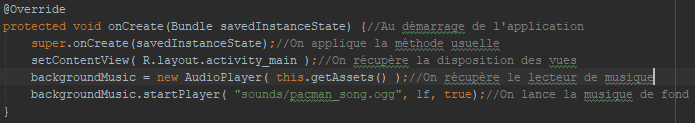
\includegraphics[scale=0.5]{MainActivity_onCreate.png}
\end{center}
Elle contient une série de méthode permettant de lancer d'autres activités, à savoir GameActivity ou ScoresActivity, ou de quitter.

\subsection{GameActivity}
\label{subsection:2_2}
GameActivity est l'activité correpondant au jeu lui-même.
\`A sa création, on récupère la location du joueur, on récupère les données de l'accéleromètre et on met l'application en plein écran.
\begin{center}
  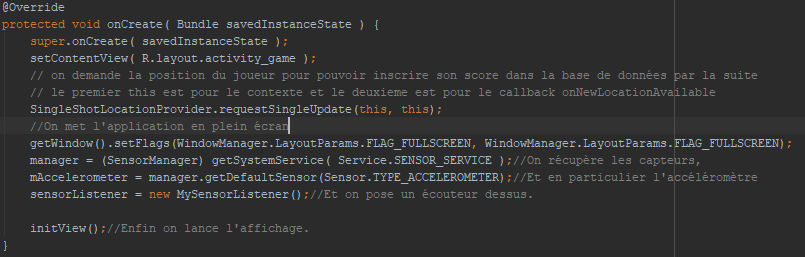
\includegraphics[scale=0.5]{GameActivity_onCreate.png}
\end{center}
Elle contient des méthodes permettant de 

\subsection{ScoresActivity}
\label{subsection:2_3}

\subsection{MapsActivityActivity}
\label{subsection:2_4}

%%% La bibliographie:
%\bibliographystyle{plain}
%\bibliography{ma_biblio}

\end{document}
%D'abord, une liste à \textbf{puces}:
%\begin{itemize}
%\item la documentation de \textit{Swing}~\cite{swingDoc}
%  est bien écrite,
%\item celle de \textit{Tkinter}~\cite{tkinterDoc} aussi!
%\end{itemize}
% \cite{...} permet de faire référence à des éléments de la
% bibliographie.

%\`A présent, une liste numérotée:
%\begin{enumerate}
%\item premier item
%\item second item
%\end{enumerate}

%\subsection{Une autre sous-section}
%Pour écrire du code, on peut par exemple utiliser l'environnement
%\textit{verbatim}:
%\begin{verbatim}
%public class Main {
%   public static void main(String[] args) {
%      System.out.println("Hello World!");
%   }
%}
%\end{verbatim}

%\section{Une autre section}

% \ref{...} permet de faire référence à un élément défini
% ailleurs dans le document (voir \label{...} plus haut).
%Contrairement à la section~\ref{section:hello},
%moi je dis: \textit{Coucou!}

%\subsection{Une sous-section}
%Voici une belle image:
%\begin{center}
%  \includegraphics[scale=0.5]{exo3_1_1.png}
%\end{center}
